\documentclass[12pt,a4paper,hidelinks]{article}
\usepackage{amsmath}
\usepackage{amsfonts}
\usepackage{amssymb}
\usepackage{makeidx}
\usepackage[left=2cm,right=2cm,top=2cm,bottom=2cm]{geometry}
\usepackage{parskip}
\usepackage{hyperref}
\usepackage{graphicx}

\usepackage{algorithm,algpseudocode}

\usepackage{listings}
\lstset{
	breaklines=true,
	tabsize=4,
	numbers=left
}

\def\algorithmautorefname{Algorithm}

\author{Bert Peters --- s1147919}
\title{Social Network Analysis for Computer Scientists --- Assignment 1}
\begin{document}

\maketitle

\section*{Exercise 1: Neighbourhoods}

\section*{Exercise 3: An Online Social Network}

\subsection*{Question 1: Number of edges}

As the file contains one link per line, the number of links can be determined by counting the number of lines. This does not require a program, but can be done with a little snippet of bash.

\lstinputlisting[language=bash]{edges.sh}

Or, rather, just use the \texttt{wc} utility. The results for this exercise are incorporated in \autoref{tab:counts}.

\subsection*{Question 2: Number of nodes}

Like for the previous exercise, a full fledged parser is still not necessary. Instead, I combine the two columns using \texttt{awk}, \texttt{sort} them, take unique rows, and finally count lines again. The exact code is shown in Listing \ref{script:nodes} and the results can be found in \autoref{tab:counts}.

\lstinputlisting[
	language=bash,
	caption=Node counter script.,
	label=script:nodes,
	float
]{nodes.sh}

The parameters for sort are slightly unusual. We do this to improve performance, so that this script can handle the \texttt{huge.in} network. The compress program allows us to use less disk space for temporaries, which is neccessary to prevent disk space issues, and we increase the buffer size to improve overall performance.

\begin{table}
\centering
\begin{tabular}{l | r | r | l | r}
Filename & {\centering $|E|$} & $-|V|$ & Directed & Largest component\\
\hline
medium.in & 16631 & 2426 & Possibly & 1998 \\
large.in & 14855842 & 456626 & Yes & 456288 \\
huge.in & 892263106 & 8113017 & Yes & 8083963
\end{tabular}
\caption{Various counts for the network files}
\label{tab:counts}
\end{table}

\subsection*{Question 3: degree distribution}

To compute the in or out degree for a node, we can simply count the number of times that a number occurs in the source or destination column. The code for this is shown in Listing \ref{script:degrees}.

\lstinputlisting[
	language=bash,
	caption=Script for computing the degree for all nodes.,
	label=script:degrees,
	float
]{degree.sh}

After we have computed the degree for various nodes, we can use this output to make a visualisation.

\lstinputlisting[
	language=python,
	caption=Degree visualizer.,
	label=script:analyze
]{analyze.py}

\begin{figure}
	\centering
	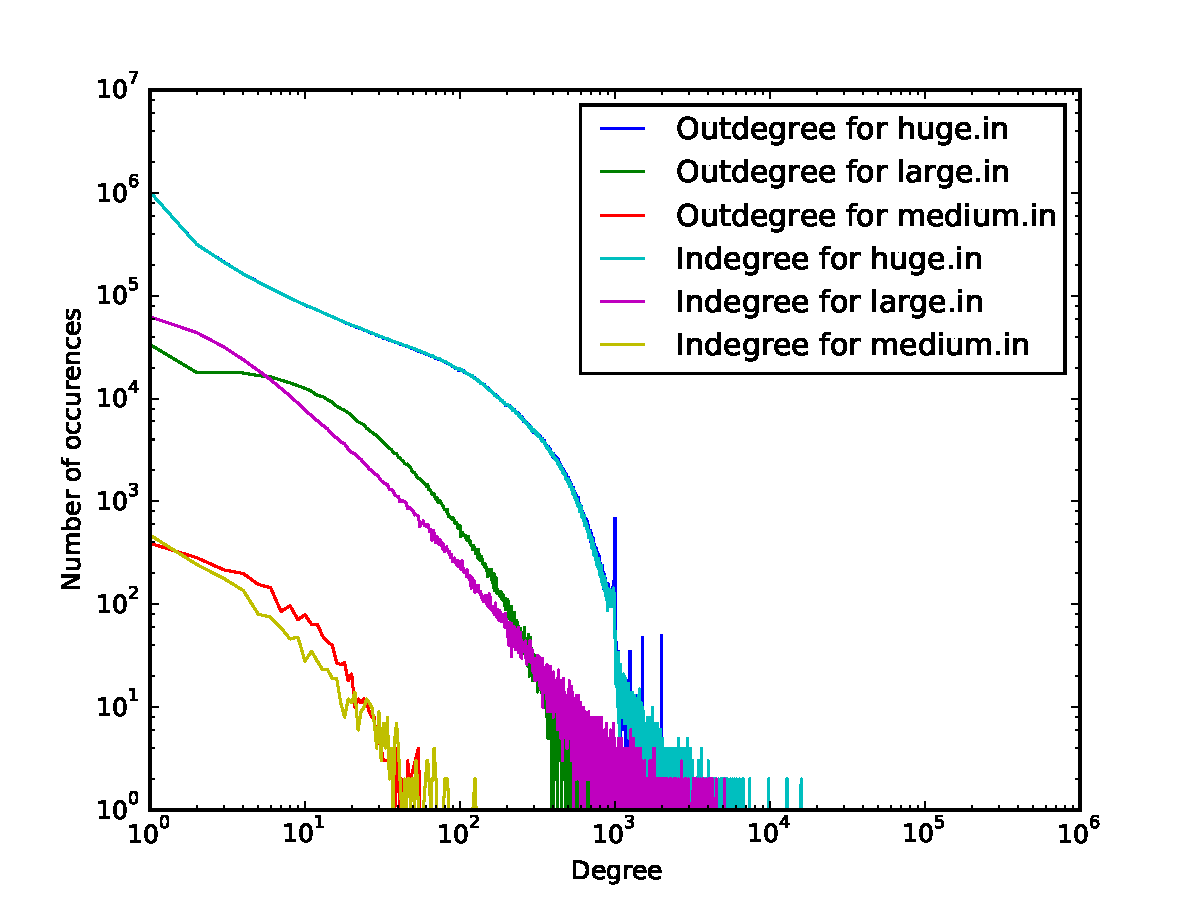
\includegraphics[scale=0.83]{degree-distributions}
	\caption{The degree distributions for all input files.}
	\label{fig:degrees}
\end{figure}

\subsection*{Question 4: directedness}

To answer this question, we must agree upon the interpretation of the file. There are some cases which can lead us to an interpretation. The following statements determine this.

\begin{align}
\label{eq:somereflex} \exists u, v &: (u, v) \in E \land (v, u) \in E \\
\label{eq:allreflex} \forall u, v &: (u, v) \in E \implies (v, u) \in E \\
\label{eq:noreflex}\nexists u, v &: (u, v) \in E \land (v, u) \in E
\end{align}

If \ref{eq:allreflex} holds, we are clearly in an undirected graph, because every edge is reflexive.

If \ref{eq:somereflex} and holds and \ref{eq:allreflex} does not, we are clearly in a directed graph because there are some reflexive connections, but not all of them are.

If, however, \ref{eq:noreflex} holds, there are no reflexive edges. This means that we can interpret the graph as either undirected or directed, because we can interpret each edge as also going back.

Once again, we implement this in bash, as it is very simple. We use \texttt{awk} to put any edge listing $(u, v)$ in the file in asceding order, so that when we sort the file, edges and returning edges are next to each other. This allows us to remove duplicates, and then analyze the number of lines that remain. We can differentiate these counts in two categories.

\begin{align*}
2 \times & |E_{unique}| = |E| & \implies & \text{Network is undirected.} \\
|E| < 2 \times & |E_{unique}| < 2 \times |E| & \implies & \text{Network is directed} \\
& |E_{unique}| = |E| & \implies & \text{Network is possibly directed}
\end{align*}

The bash script in Listing \ref{script:directed} computes $|E|$ and $|E_{unique}|$ and prints out the category the network falls in.

\lstinputlisting[
	language=bash,
	caption=Code that computes whether or not a graph is directed,
	label=script:directed,
	float
]{directed.sh}

\subsection*{Question 3.5: Largest connected component}

For this section, we consider the largest connected component to be the largest weakly connected component. This helps us, because this removes the distinction between directed and undirected networks.

To compute the largest connected component, I could not come up with a \texttt{bash}-based solution, so I reverted to using \texttt{C++}.

The algorithm works as follows. First, we store our edges into a large edge array and sort them on $u, v$. After that, we attempt to make a coloring for each node. In this coloring, connected nodes are the same color. Finally, we determine the number of occurences for the most frequent color. This is our answer. The code for this algorithm can be found in \autoref{appendix:components}.

\subsubsection*{Coloring algorithm}

The coloring algorithm is more or less a breadth first search, as described in \autoref{algo:coloring}. We know that the complexity of a breadth first search is $O(|E|)$,\footnote{Technically, this is $|V|)$, but because we consider sparse networks, $|E| \approx |V|$ so we ignore $|E|$. This simplifies our formulae.} without accounting for the complexity of determining neighbours for nodes. Because we sorted our list of edges, we can access the neighbours of $u$ using binary search in $O(B + \log |E|)$, with $B$ the number of neighbours.

In the inner loop of our algorithm, the most complex task we potentially do, is recoloring all the nodes. The way we do this is enumerating all nodes and replacing the colors we have to. This is an $O(|V|)$ operation. This happens each time we find a new directed route into an existing component. However, this rarely happens. Most of the time, we find a connected component once, because the networks are very reflexive.

So, to summarize, our theorethical complexity is $O(|V|(\log |E| + |V|))$.\footnote{We ignore the $B$ in the complexity for accessing neighbours, because the rest of the loop gets executed just as often. Therefore, it is already part of the BFS complexity.} This works out to $O(|V|^2 + |V|\log|E|) \approx O(|V|^2)$. This complexity however includes the recoloring cost, so while it is the worst case, the average case is better, and runs in $O(|V| \log |E|)$.

\begin{algorithm}
\caption{Node coloring algorithm}
\label{algo:coloring}
\begin{algorithmic}

\ForAll{$u \in V$}
	\State initialize $color_u$ as 0
\EndFor
\\
\ForAll{$u \in V$}
	\If{$color_u = 0$}
		\State $todo \gets \{u\}$
		\While{$todo \neq \emptyset$}
			\State Pick a $v$ from $todo$
			\State $todo \gets todo \setminus \{v\}$
			\If{$color_v \neq u$}
				\If{$color_v = 0$}
					\State $color_v \gets u$
					\State Add all $w : w \in N_1(v) \land  color_w \neq u$ to $todo$.
				\Else
					\State Recolor all $w : color_w = color_v$ to $u$.
				\EndIf
			\EndIf
		\EndWhile
	\EndIf
\EndFor

\end{algorithmic}
\end{algorithm}

\appendix

\section{Source listing for component.cpp}
\label{appendix:components}

Below is the source for \texttt{component.cpp}. The program was compiled using \texttt{g++ -std=c++11 -O2}.

\lstinputlisting[language=c++]{component.cpp}

\end{document}
